\documentclass{article}

\usepackage{graphicx}

\title{Problem7 Report}
\author{Qi Liu}
\date{\today}

\begin{document}

\maketitle

\section{Discrete Cosine Transform Compression}
Here we use discrete cosine transform (DCT) to compress the iamge. First we split the input image to multiple $8\times 8$ sub-images and apply DCT on the sub-images. Then we truncate the DCT coefficients with some mask and reconstruct the image by using inverse DCT on the sub-images. 

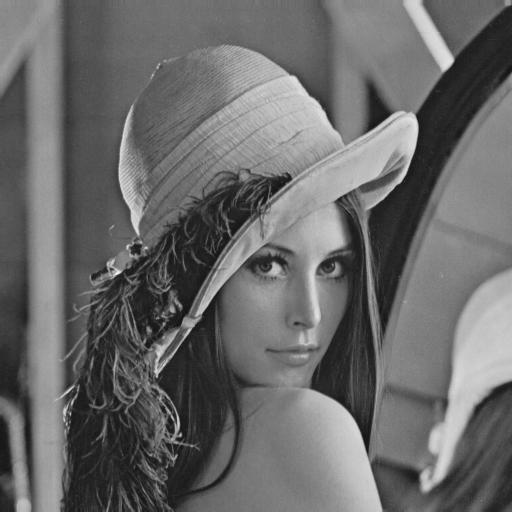
\includegraphics[width=0.33\textwidth]{../data/lenna.jpg}
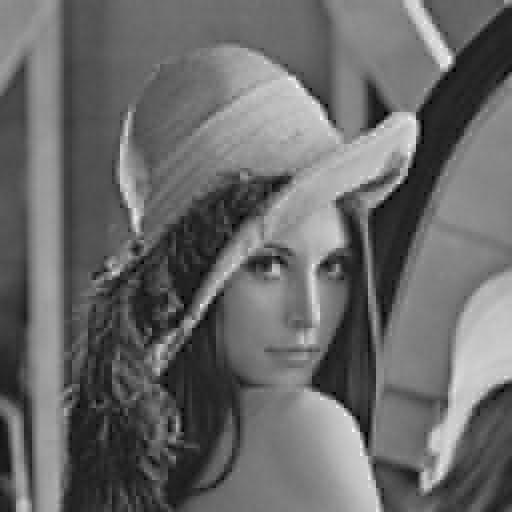
\includegraphics[width=0.33\textwidth]{../data/zonal_1_lenna.jpg}
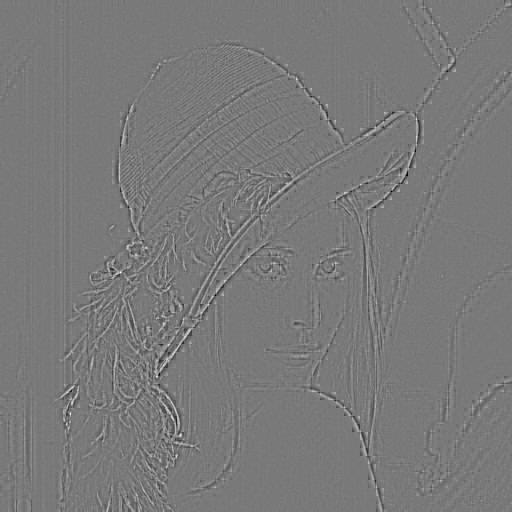
\includegraphics[width=0.33\textwidth]{../data/delta_zonal_1_lenna.jpg}

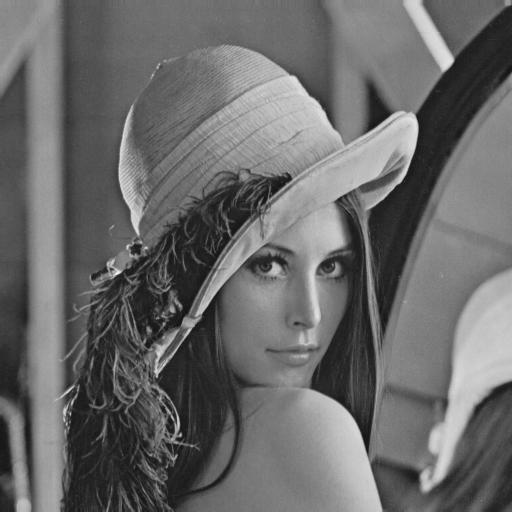
\includegraphics[width=0.33\textwidth]{../data/lenna.jpg}
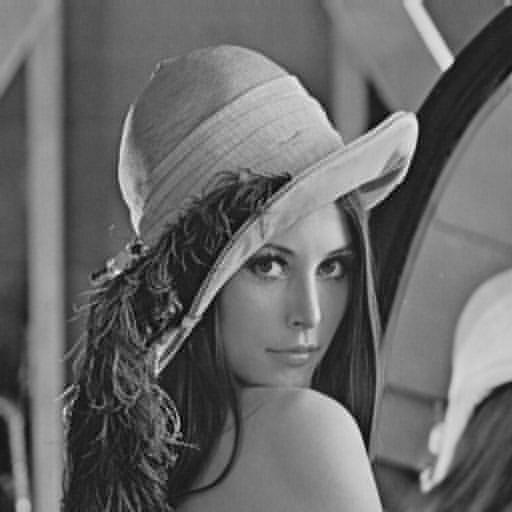
\includegraphics[width=0.33\textwidth]{../data/zonal_3_lenna.jpg}
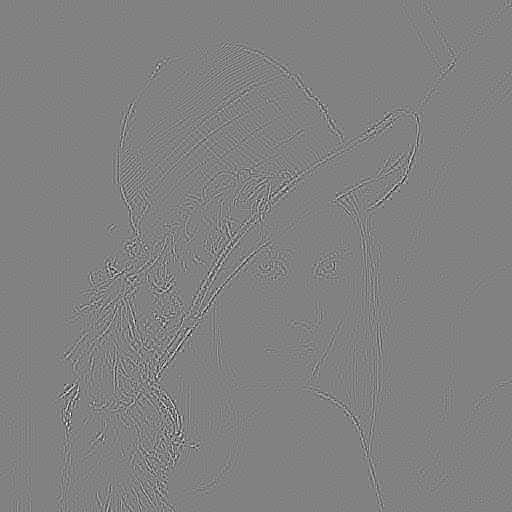
\includegraphics[width=0.33\textwidth]{../data/delta_zonal_3_lenna.jpg}

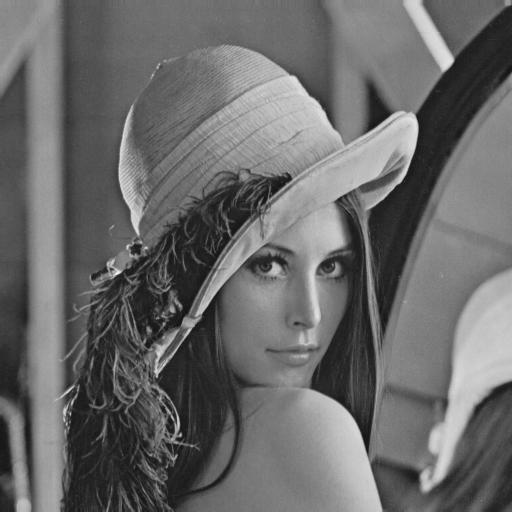
\includegraphics[width=0.33\textwidth]{../data/lenna.jpg}
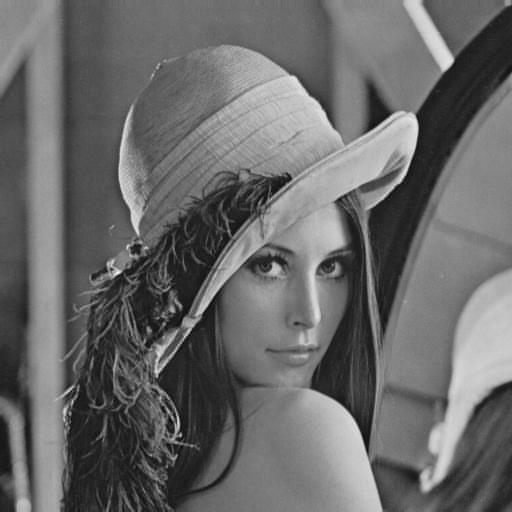
\includegraphics[width=0.33\textwidth]{../data/zonal_5_lenna.jpg}

\includegraphics[width=0.33\textwidth]{../data/delta_zonal_5_lenna.jpg}

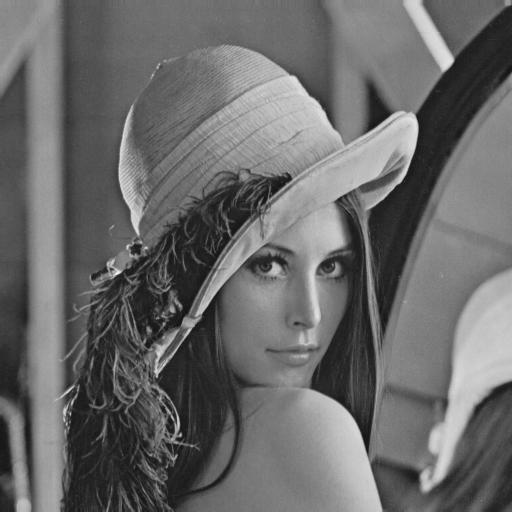
\includegraphics[width=0.33\textwidth]{../data/lenna.jpg}
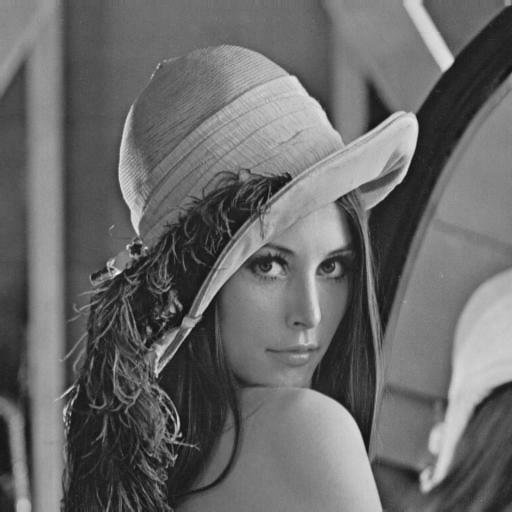
\includegraphics[width=0.33\textwidth]{../data/zonal_7_lenna.jpg}

\includegraphics[width=0.33\textwidth]{../data/delta_zonal_7_lenna.jpg}

The figures above are the results of using zonal mask. From the first row to the fourth row, the zonal mask contains 2, 4, 6 and 8 anti-diagonals from the up-left corner, the compression ratio are 4.6875\%, 15.625\%, 32.8125\% and 56.25\% respectively. For every row, the first is the original image, the second is the compression image and the third is the delta image.

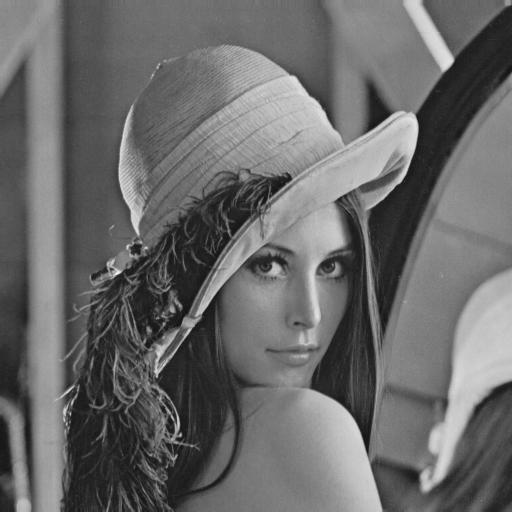
\includegraphics[width=0.33\textwidth]{../data/lenna.jpg}
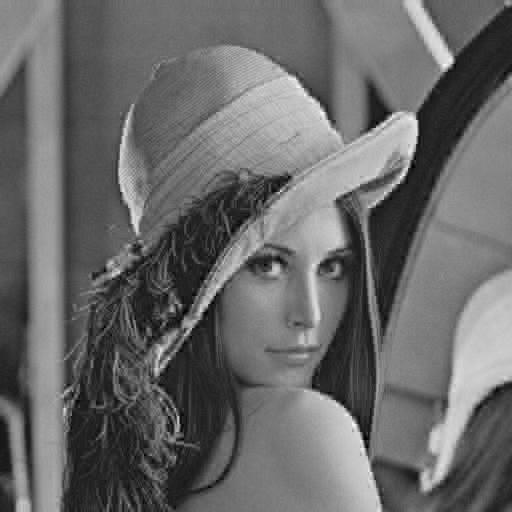
\includegraphics[width=0.33\textwidth]{../data/threshold_4_lenna.jpg}
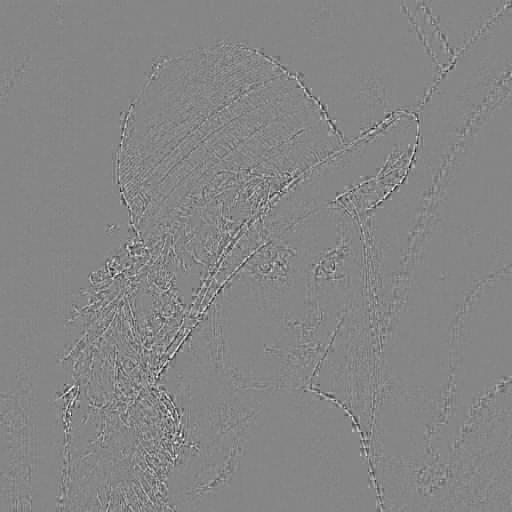
\includegraphics[width=0.33\textwidth]{../data/delta_threshold_4_lenna.jpg}

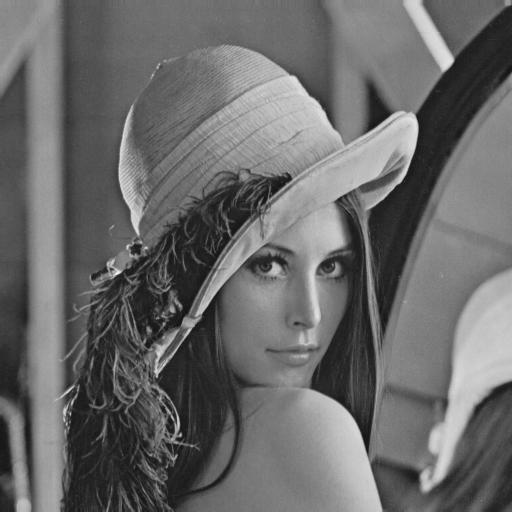
\includegraphics[width=0.33\textwidth]{../data/lenna.jpg}
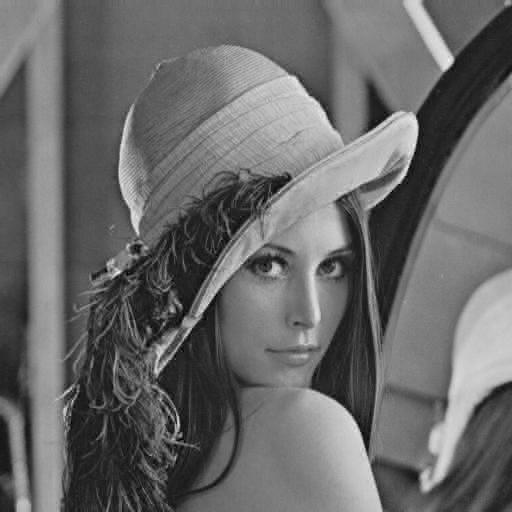
\includegraphics[width=0.33\textwidth]{../data/threshold_8_lenna.jpg}
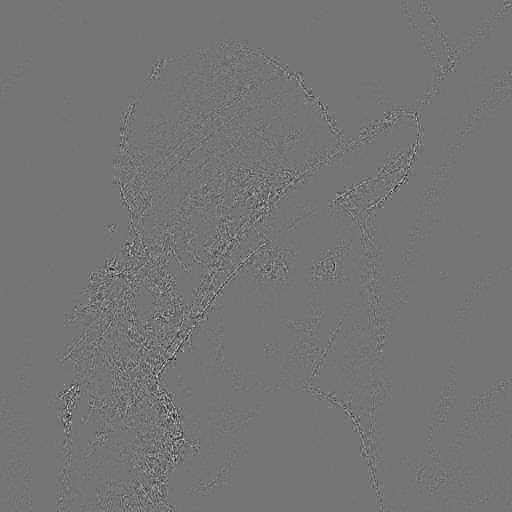
\includegraphics[width=0.33\textwidth]{../data/delta_threshold_8_lenna.jpg}

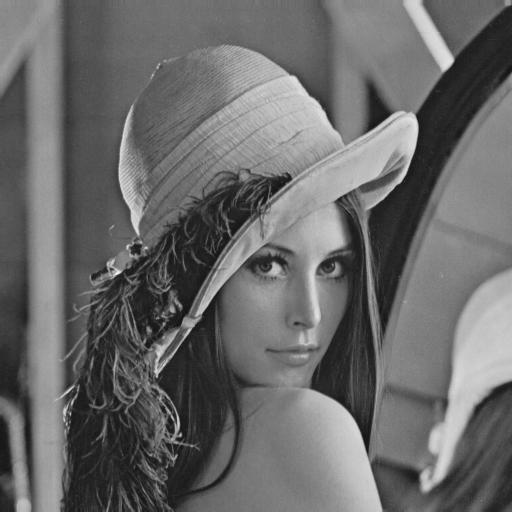
\includegraphics[width=0.33\textwidth]{../data/lenna.jpg}
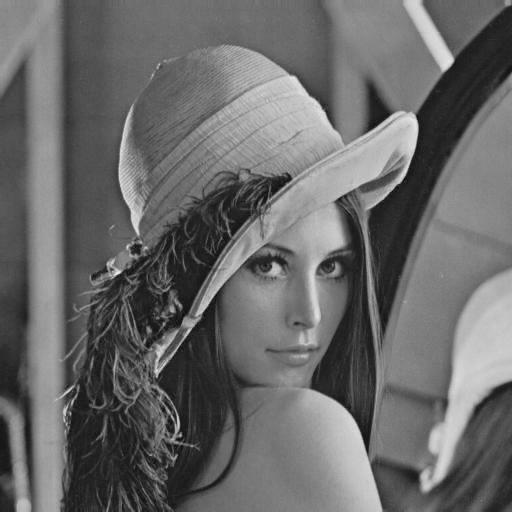
\includegraphics[width=0.33\textwidth]{../data/threshold_16_lenna.jpg}
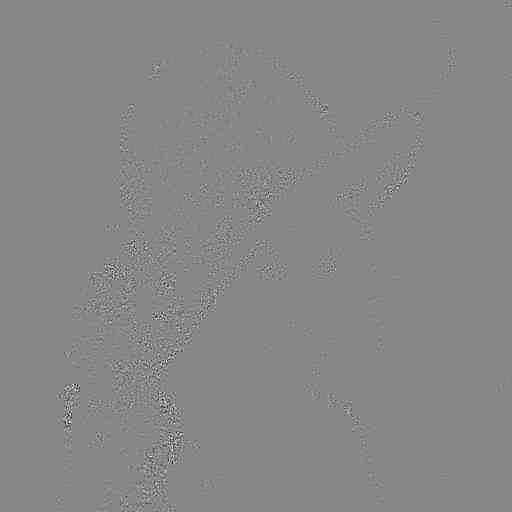
\includegraphics[width=0.33\textwidth]{../data/delta_threshold_16_lenna.jpg}

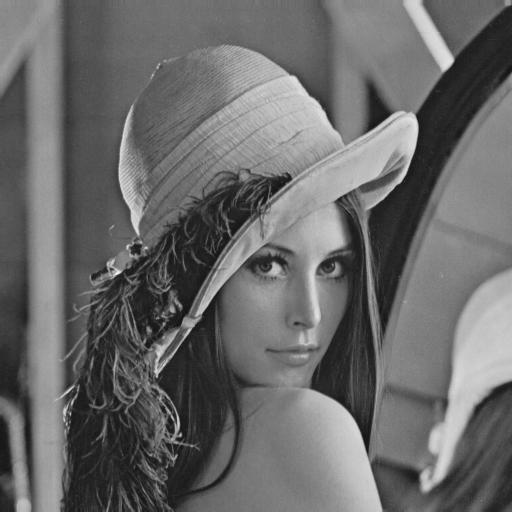
\includegraphics[width=0.33\textwidth]{../data/lenna.jpg}
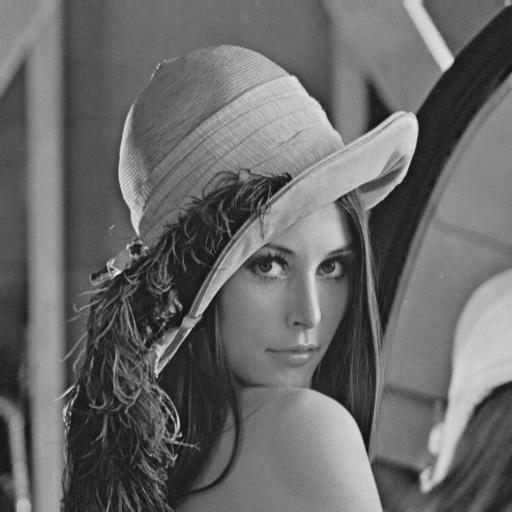
\includegraphics[width=0.33\textwidth]{../data/threshold_32_lenna.jpg}
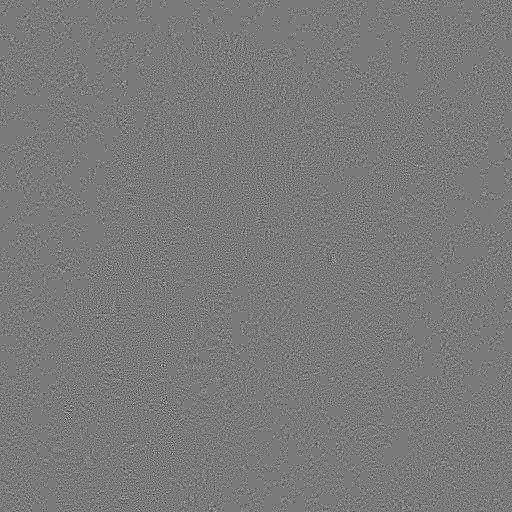
\includegraphics[width=0.33\textwidth]{../data/delta_threshold_32_lenna.jpg}

The figures above are the results of using threshold mask. From the first row to the fourth row, the threshold mask contains the largest 4, 8, 16 and 32 coefficients, the compression ratio are 6.25\%, 12.5\%, 25\% and 50\% respectively. For every row, the first is the original image, the second is the compression image and the third is the delta image.

\section{Wavelet Transform Compression}
We use four kinds of wavelet to do wavelet transform compression. Their coefficients are shown below.
$$\textbf{Haar}: h_0=[\frac{1}{\sqrt{2}},\frac{1}{\sqrt{2}}], h1=[\frac{1}{\sqrt{2}},-\frac{1}{\sqrt{2}}]$$
$$\textbf{Daubechies}:
\begin{tabular}{|c|c|}
	\hline $n$&$g_0(n)$\\
	\hline
	0&0.23037781 \\
	1&0.71484657 \\
	2&0.63088076 \\
	3&-0.02798376 \\
	4&-0.18703481 \\
	5&0.03084138 \\
	6&0.03288301 \\
	7&-0.01059740 \\
	\hline
\end{tabular}
\quad \textbf{Symlet}:
\begin{tabular}{|c|c|}
	\hline $n$&$g_0(n)$\\
	\hline 
	0&0.0322 \\
	1&-0.0126 \\
	2&-0.0992 \\
	3&0.2979 \\
	4&0.8037 \\
	5&0.4976 \\
	6&-0.0296 \\
	7&-0.0758 \\
	\hline
\end{tabular}
$$
$$
\textbf{Cohen-Daubechies-Feauveau}:
\begin{tabular}{|c|cc|c|cc|}
	\hline $n$&$h_0(n)$&$h_1(n)$&$n$&$h_0(n)$&$h_1(n)$\\
	\hline
	0&0&0&9&0.8259&0.4178 \\
	1&0.0019&0&10&0.4208&0.0404 \\
	2&-0.0019&0&11&-0.0941&-0.0787 \\
	3&-0.017&0.0144&12&-0.0773&-0.0145 \\
	4&0.0119&-0.0145&13&0.0497&0.0144 \\
	5&0.0497&-0.0787&14&0.0119&0 \\
	6&-0.0773&0.0404&15&-0.017&0 \\
	7&-0.0941&0.4178&16&-0.0019&0 \\
	8&0.4208&-0.7589&17&0.0010&0 \\
	\hline 
\end{tabular}
$$

The figures below are the results of wavelet transform compression.
The first row to the fourth row are the results of using Haar wavelet, Daubechies wavelet, Symlet wavelet and Cohen-Daubechies-Feauveau wavelet. We truncated the wavelet transform coefficients less than one to zero. The compression ratio are 43.3\%, 48.5\%, 51.3\% and 53.7\% respectively. For every row, the first one is the original image, the second one is the wavelet transform image, the third one is the compression image and the fourth one is the delta image.

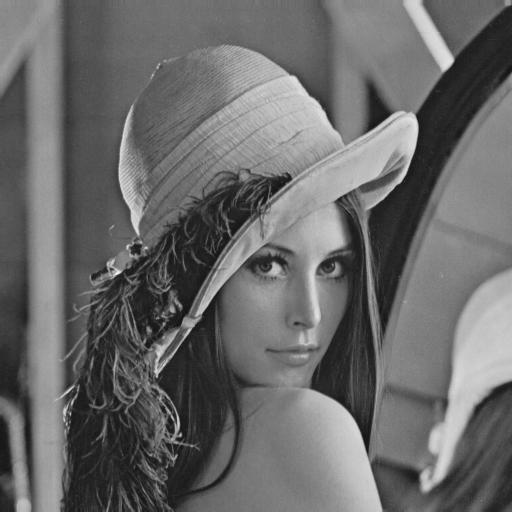
\includegraphics[width=0.25\textwidth]{../data/lenna.jpg}
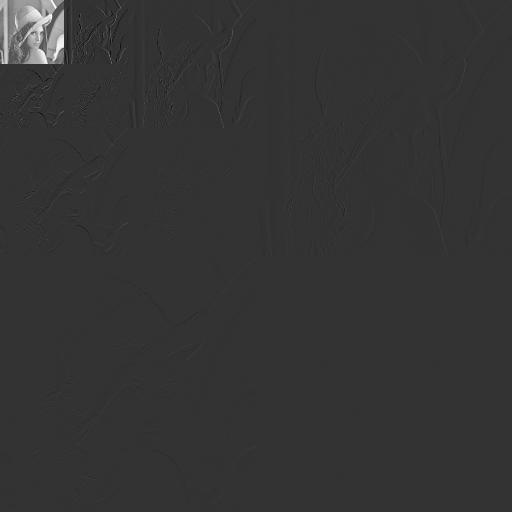
\includegraphics[width=0.25\textwidth]{../data/haar_transform_lenna.jpg}
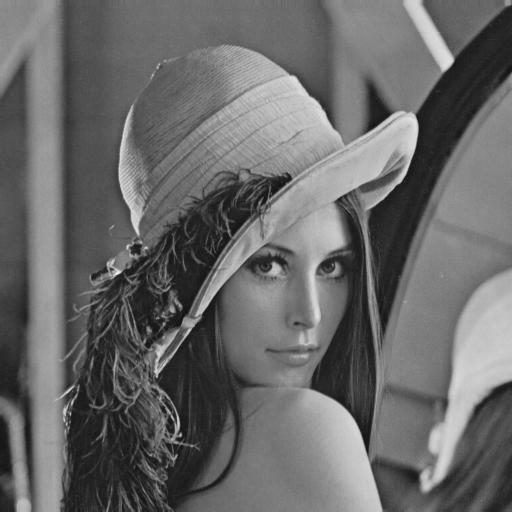
\includegraphics[width=0.25\textwidth]{../data/haar_lenna.jpg}
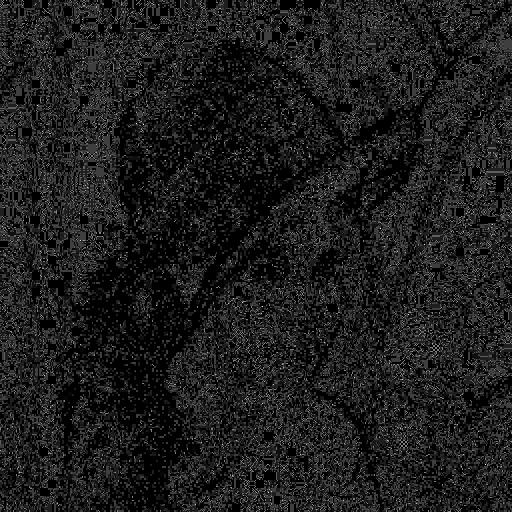
\includegraphics[width=0.25\textwidth]{../data/delta_haar_lenna.jpg}

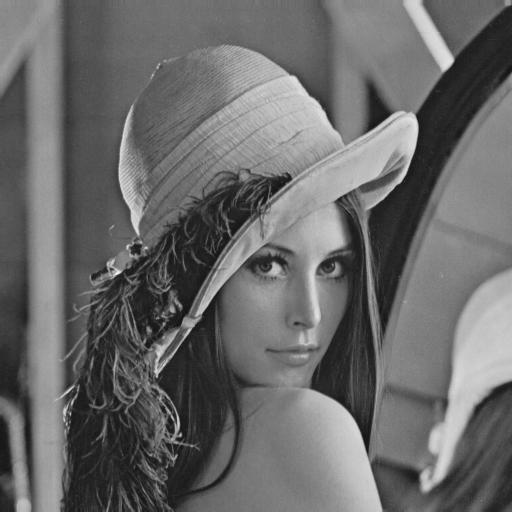
\includegraphics[width=0.25\textwidth]{../data/lenna.jpg}
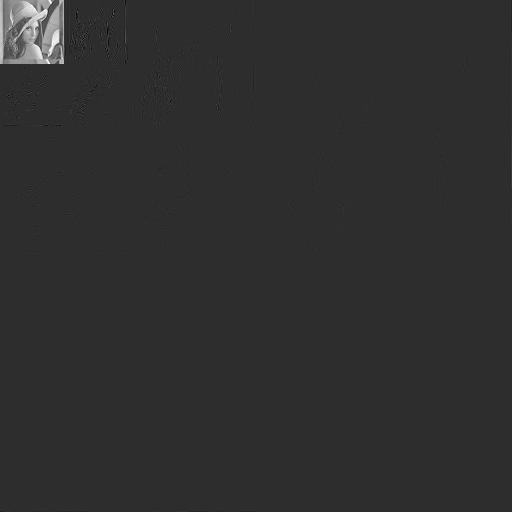
\includegraphics[width=0.25\textwidth]{../data/daubechies_transform_lenna.jpg}
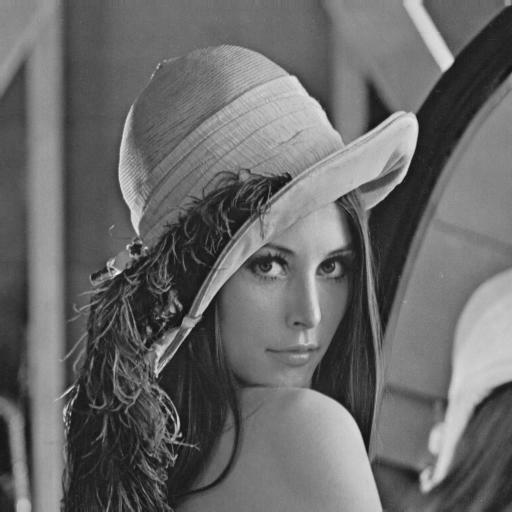
\includegraphics[width=0.25\textwidth]{../data/daubechies_lenna.jpg}
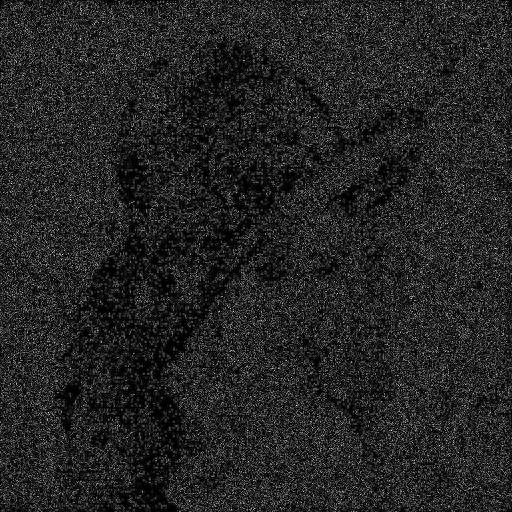
\includegraphics[width=0.25\textwidth]{../data/delta_daubechies_lenna.jpg}

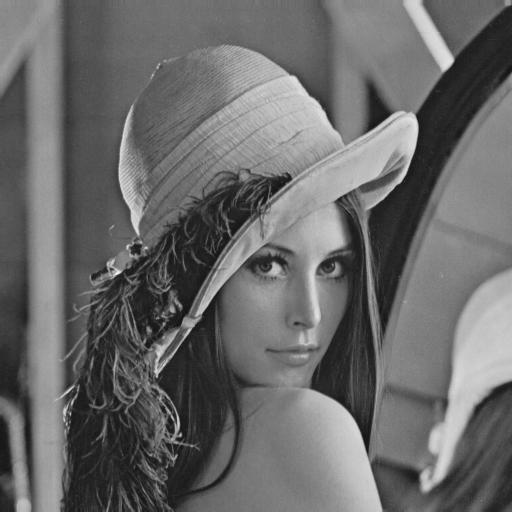
\includegraphics[width=0.25\textwidth]{../data/lenna.jpg}
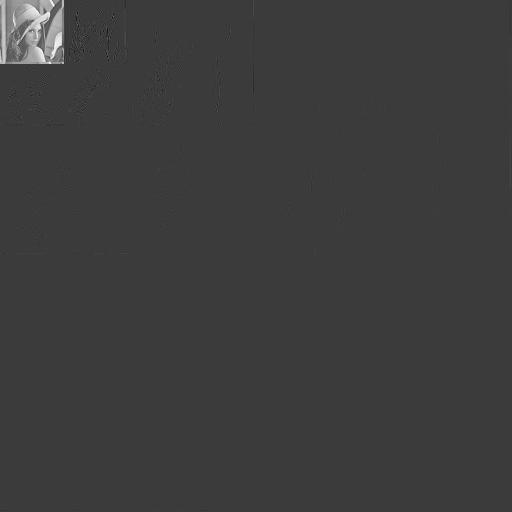
\includegraphics[width=0.25\textwidth]{../data/symlet_transform_lenna.jpg}
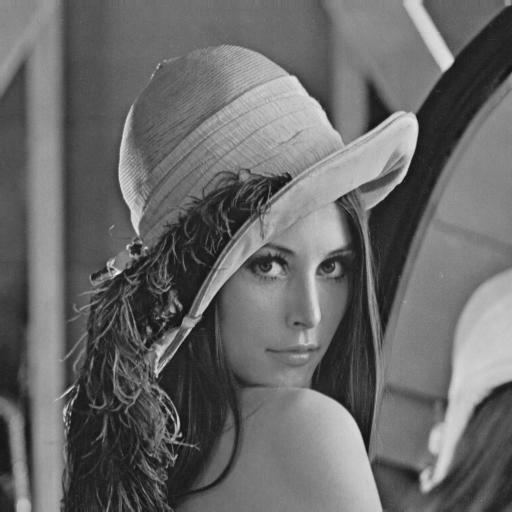
\includegraphics[width=0.25\textwidth]{../data/symlet_lenna.jpg}
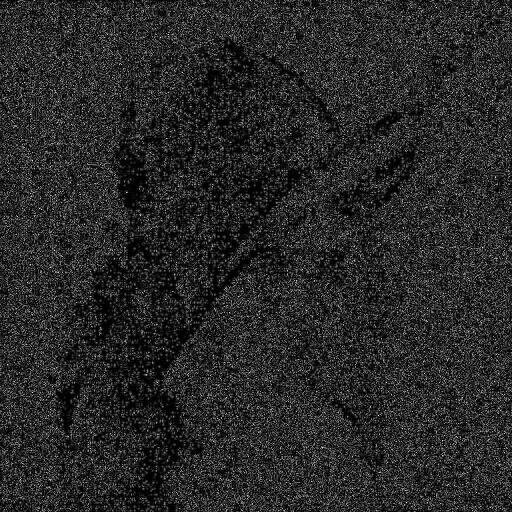
\includegraphics[width=0.25\textwidth]{../data/delta_symlet_lenna.jpg}

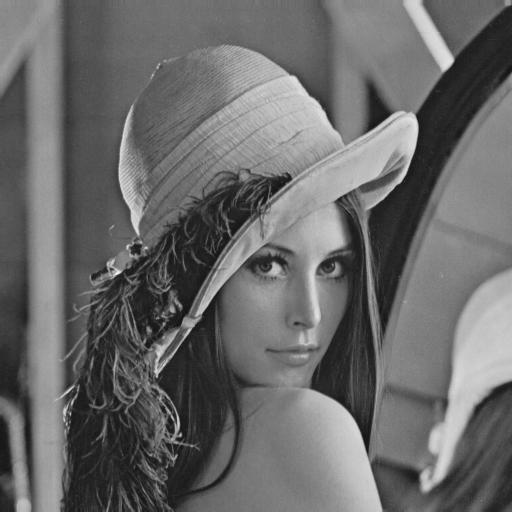
\includegraphics[width=0.25\textwidth]{../data/lenna.jpg}
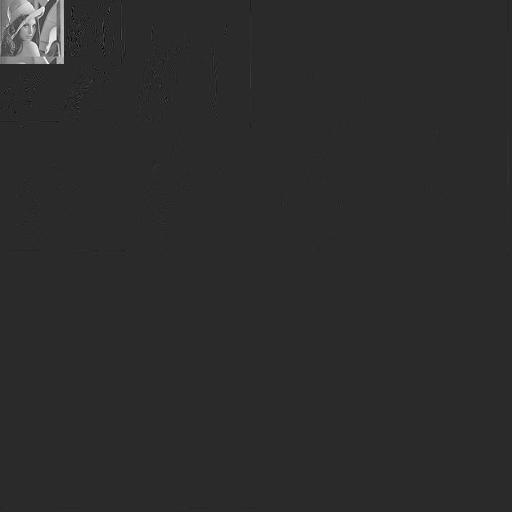
\includegraphics[width=0.25\textwidth]{../data/cohen_daubechies_feauveau_transform_lenna.jpg}
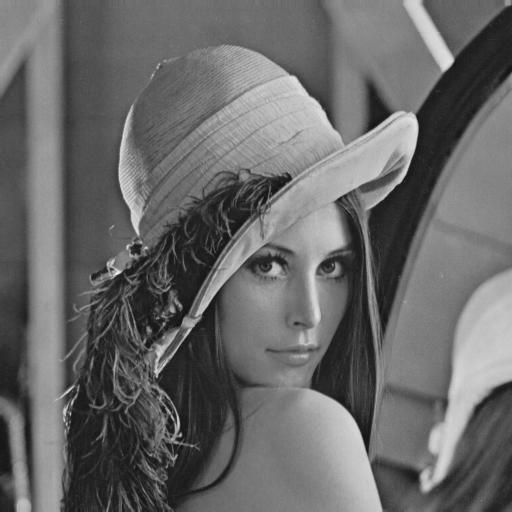
\includegraphics[width=0.25\textwidth]{../data/cohen_daubechies_feauveau_lenna.jpg}
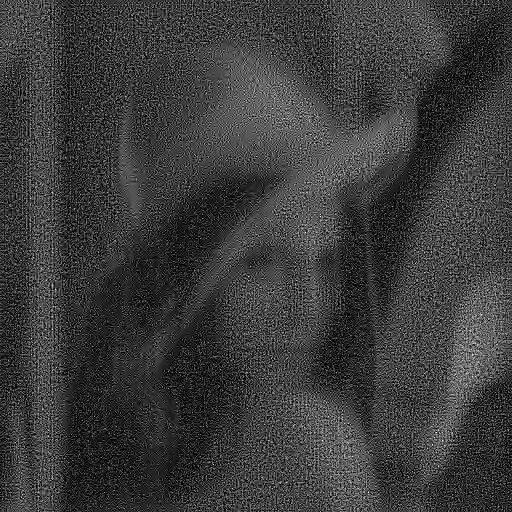
\includegraphics[width=0.25\textwidth]{../data/delta_cohen_daubechies_feauveau_lenna.jpg}

\end{document}